\documentclass{article}

\usepackage{arxiv}

\usepackage[utf8]{inputenc} % allow utf-8 input
\usepackage[T1]{fontenc}    % use 8-bit T1 fonts
\usepackage{hyperref}       % hyperlinks
\usepackage{url}            % simple URL typesetting
\usepackage{booktabs}       % professional-quality tables
\usepackage{amsfonts}       % blackboard math symbols
\usepackage{nicefrac}       % compact symbols for 1/2, etc.
\usepackage{microtype}      % microtypography
\usepackage{graphicx}
\graphicspath{ {./images/} }

\title{Parkinson's Disease Classification from Handwriting Time Series}

\author{
 Stefano \\
  Department of Computer Science \\
  University of Bari Aldo Moro \\
  Bari, Italy \\
  \texttt{email@institution.it} \\
}

\begin{document}
\maketitle

\begin{abstract}
This project aims to build a binary classification model to distinguish between Parkinson's disease (PD) patients and healthy control (H) subjects using the PaHaW Handwriting Dataset. By extracting statistical and dynamic features from the raw time-series data, we trained a Random Forest Classifier. The optimized baseline model achieves an accuracy of approximately 66.7\% and an AUC of 0.71, demonstrating the feasibility of using digitizing tablet data for neurodegenerative disease screening.
\end{abstract}

\section{Introduction}
Parkinson's disease (PD) is a progressive neurodegenerative disorder that affects movement, often including symptoms such as tremors, rigidity, and bradykinesia. One of the earliest and most noticeable manifestations of PD is a change in handwriting, commonly resulting in micrographia (abnormally small handwriting). This study aims to build a binary classification model to distinguish between PD patients and healthy control subjects using time-series handwriting data. Developing a reliable, automated screening tool could facilitate early diagnosis and continuous monitoring of the disease using non-invasive techniques.

\section{Related Work}
Previous research has extensively investigated the application of machine learning techniques for the early diagnosis of Parkinson's disease using various modalities, including voice recordings, gait analysis, and handwriting. In the domain of handwriting analysis, studies have shown that dynamic features such as pen pressure, velocity, and in-air movements are strong indicators of PD. While recent advancements employ complex Convolutional Neural Networks (CNNs) on visual representations of time series (e.g., spectrograms), traditional machine learning models like Random Forests remain highly effective baselines for tabular statistical aggregates, especially when dealing with small datasets where deep learning is prone to overfitting.

\section{Materials}
The dataset used in this study is the \textbf{Parkinson's Disease Handwriting Database (PaHaW)}. It consists of time-series data captured from a digitizing tablet, measuring variables like X and Y coordinates, pen pressure, altitude, azimuth, and button state (indicating whether the pen touches the surface). 

During data preprocessing, subjects \texttt{00061}, \texttt{00080}, and \texttt{00089} were safely removed prior to feature extraction as they did not complete all tasks. The remaining data comprises 72 subjects. We mapped the target variable \texttt{Disease} into binary labels: 'PD' (labeled 1) and 'H' (labeled 0). 

\section{Methods}
The methodology relies on robust feature engineering followed by a standard machine learning classifier.
\begin{itemize}
    \item \textbf{Feature Engineering}: For each patient's handwriting task files, we extracted statistical metrics (mean, standard deviation, max, min, median) for physical properties (X, Y, Altitude, Azimuth, Pressure), temporal features (total duration), and dynamic features (continuous velocity derived from spatial displacement and time deltas).
    \item \textbf{Aggregation}: These features were averaged across all handwriting tasks per subject, resulting in a single high-dimensional feature vector per person.
    \item \textbf{Modeling}: We used a \texttt{RandomForestClassifier} with optimized hyperparameters (\texttt{n\_estimators=200}, \texttt{max\_depth=7}, \texttt{min\_samples\_split=5}) to prevent overfitting and improve precision. The dataset was split into 80/20 Train-Test subsets, and we applied Stratified 5-Fold Cross Validation on the training set for robust validation.
\end{itemize}

\section{Results}
The optimized baseline model achieves an accuracy of approximately \textbf{66.7\%} with an AUC of \textbf{0.71}. Table~\ref{tab:metrics} presents the complete evaluation metrics on the hold-out test set.

\begin{table}[h]
 \caption{Hold-Out Test Set Evaluation Metrics}
  \centering
  \begin{tabular}{ll}
    \toprule
    Metric & Value (\%) \\
    \midrule
    Accuracy & 66.7 \\
    Precision & 62.5 \\
    Recall & 71.4 \\
    Specificity & 62.5 \\
    F1-Score & 66.7 \\
    \bottomrule
  \end{tabular}
  \label{tab:metrics}
\end{table}

The model demonstrates a good balance between identifying Parkinson's patients (Recall: 71.4\%) and healthy control subjects. The most discriminative features identified by the Random Forest include the median and mean values of the X and Y coordinates, highlighting the importance of spatial positioning in the handwriting task.

Figure~\ref{fig:feature_importances} illustrates the top 10 most discriminative features. Figure~\ref{fig:confusion_matrix} provides a detailed view of the True Positives, True Negatives, False Positives, and False Negatives, giving insight into the model's performance in distinguishing the two classes. Finally, Figure~\ref{fig:roc_curve} plots the ROC curve, visualizing the trade-off between sensitivity and specificity alongside the calculated AUC score of 0.71.

\begin{figure}[htbp]
    \centering
    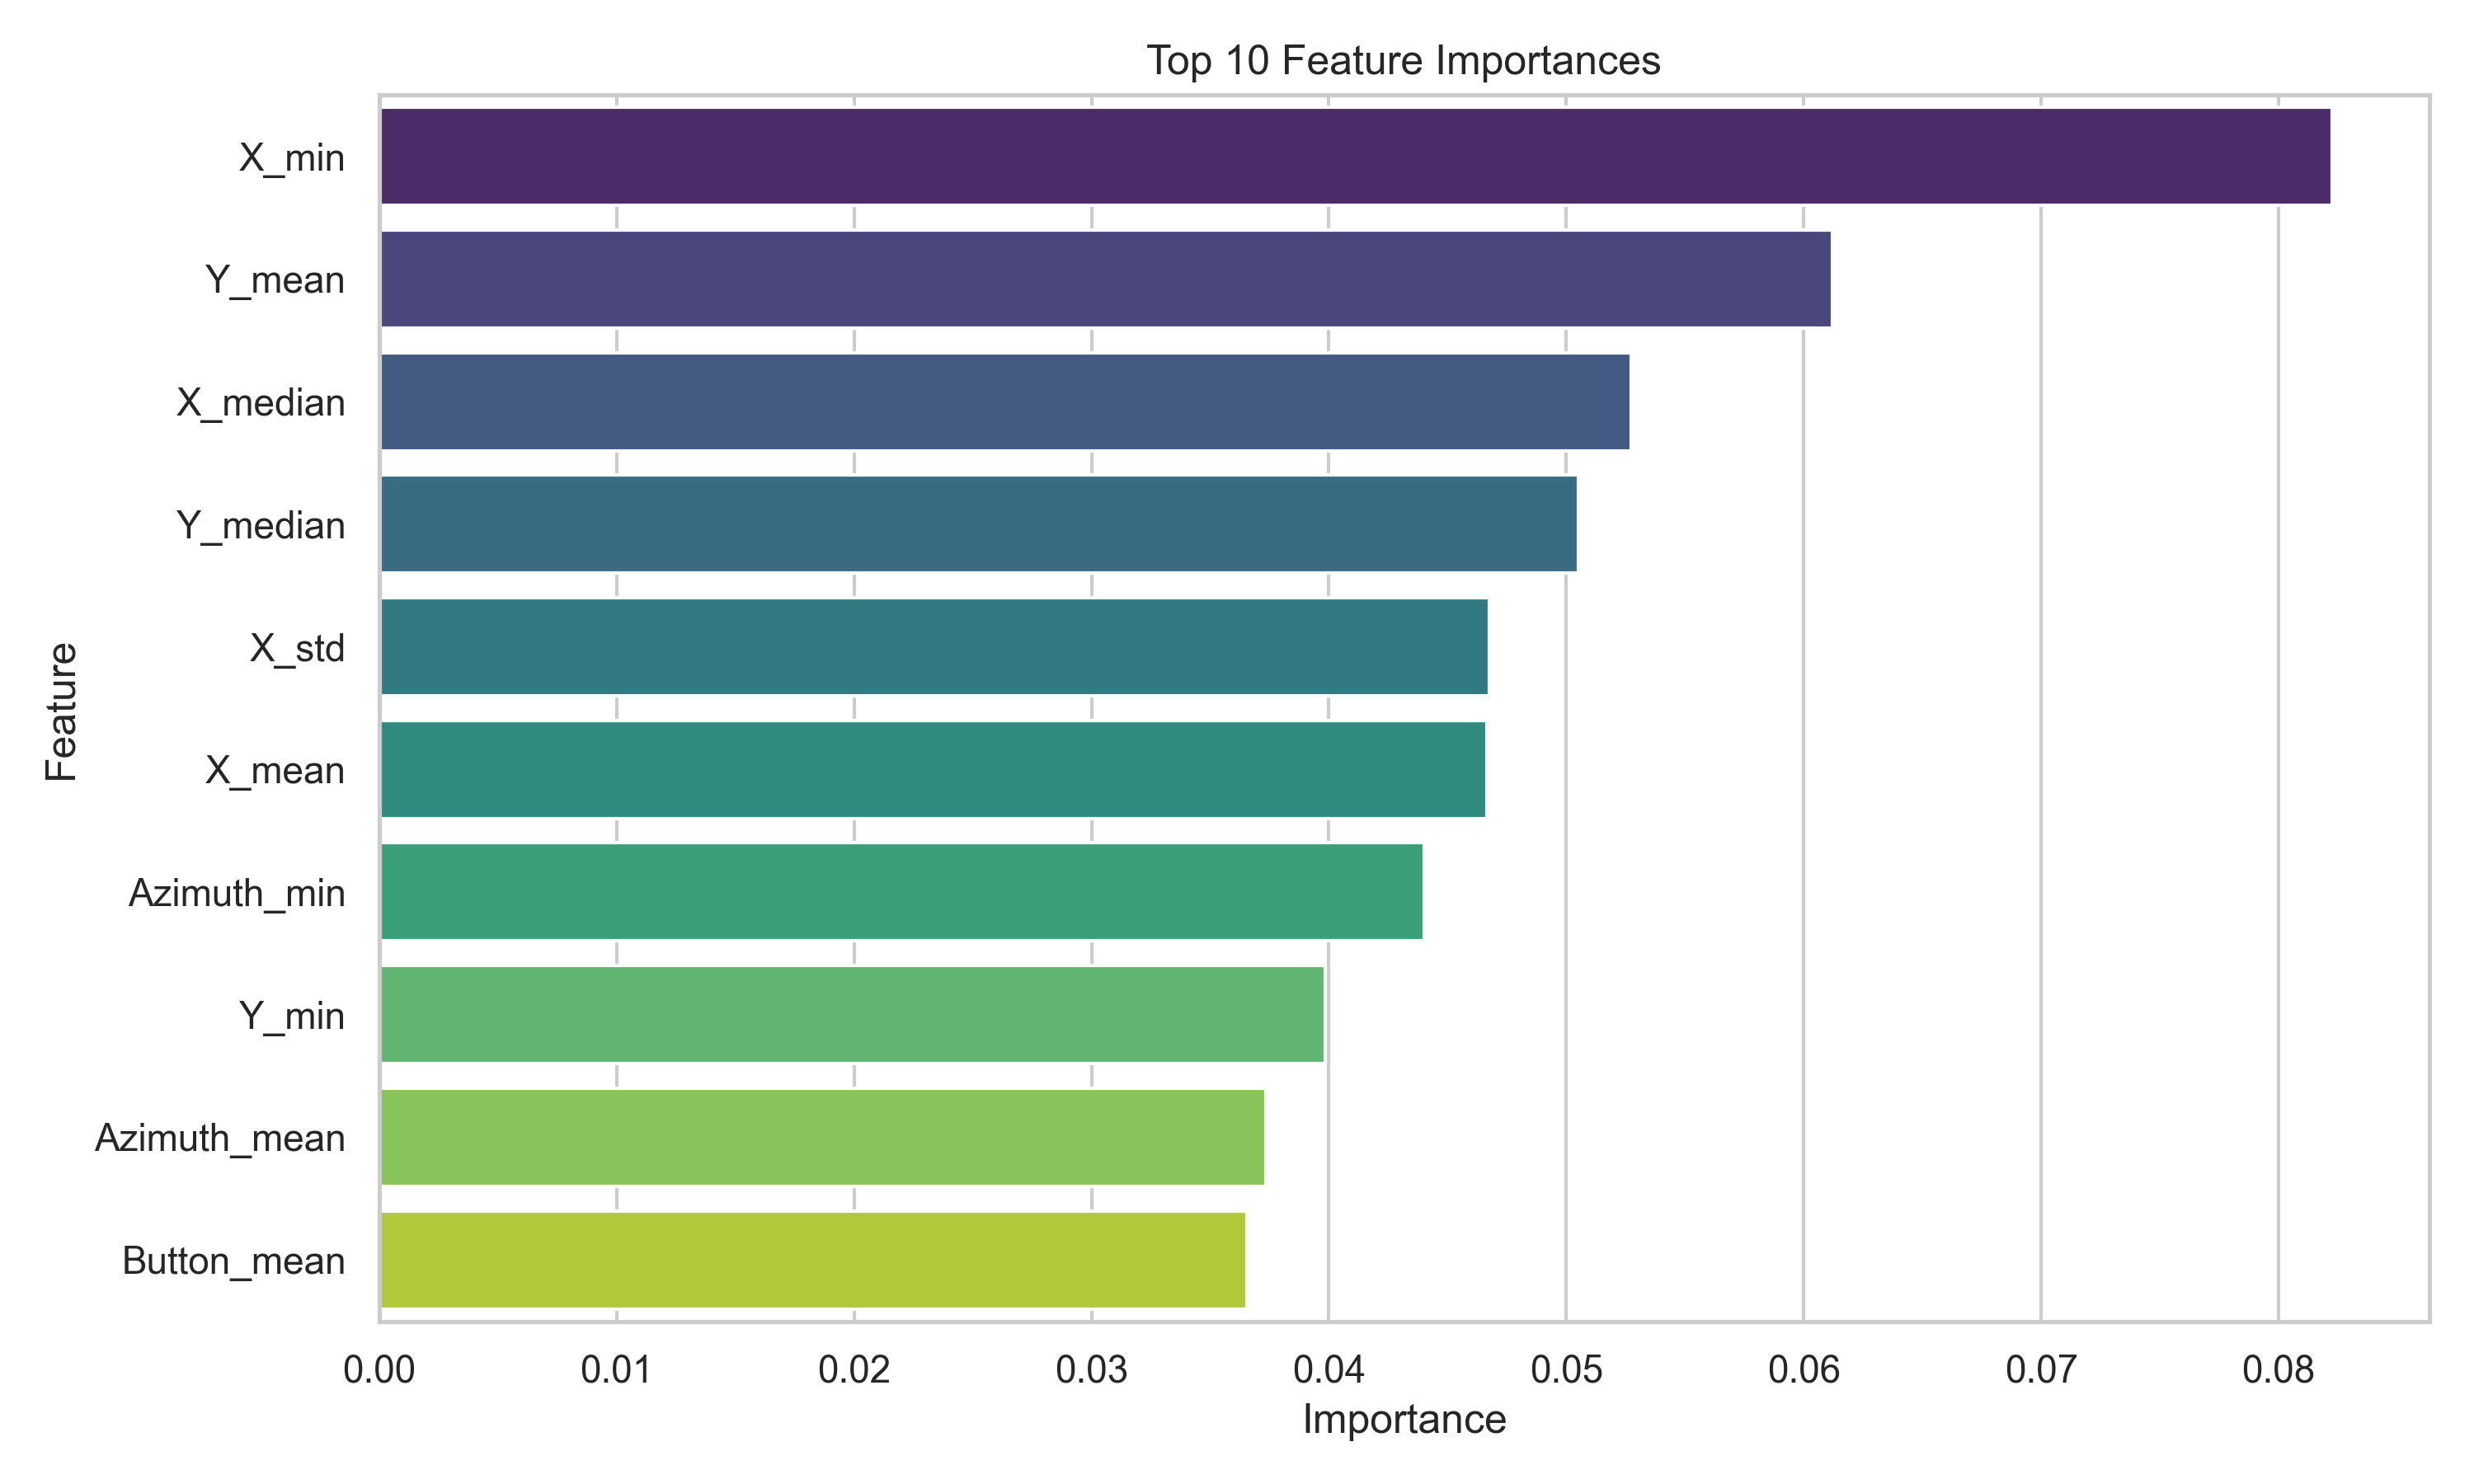
\includegraphics[width=0.8\textwidth]{feature_importances.png}
    \caption{Top 10 Feature Importances identified by the Random Forest model.}
    \label{fig:feature_importances}
\end{figure}

\begin{figure}[htbp]
    \centering
    \begin{minipage}{0.48\textwidth}
        \centering
        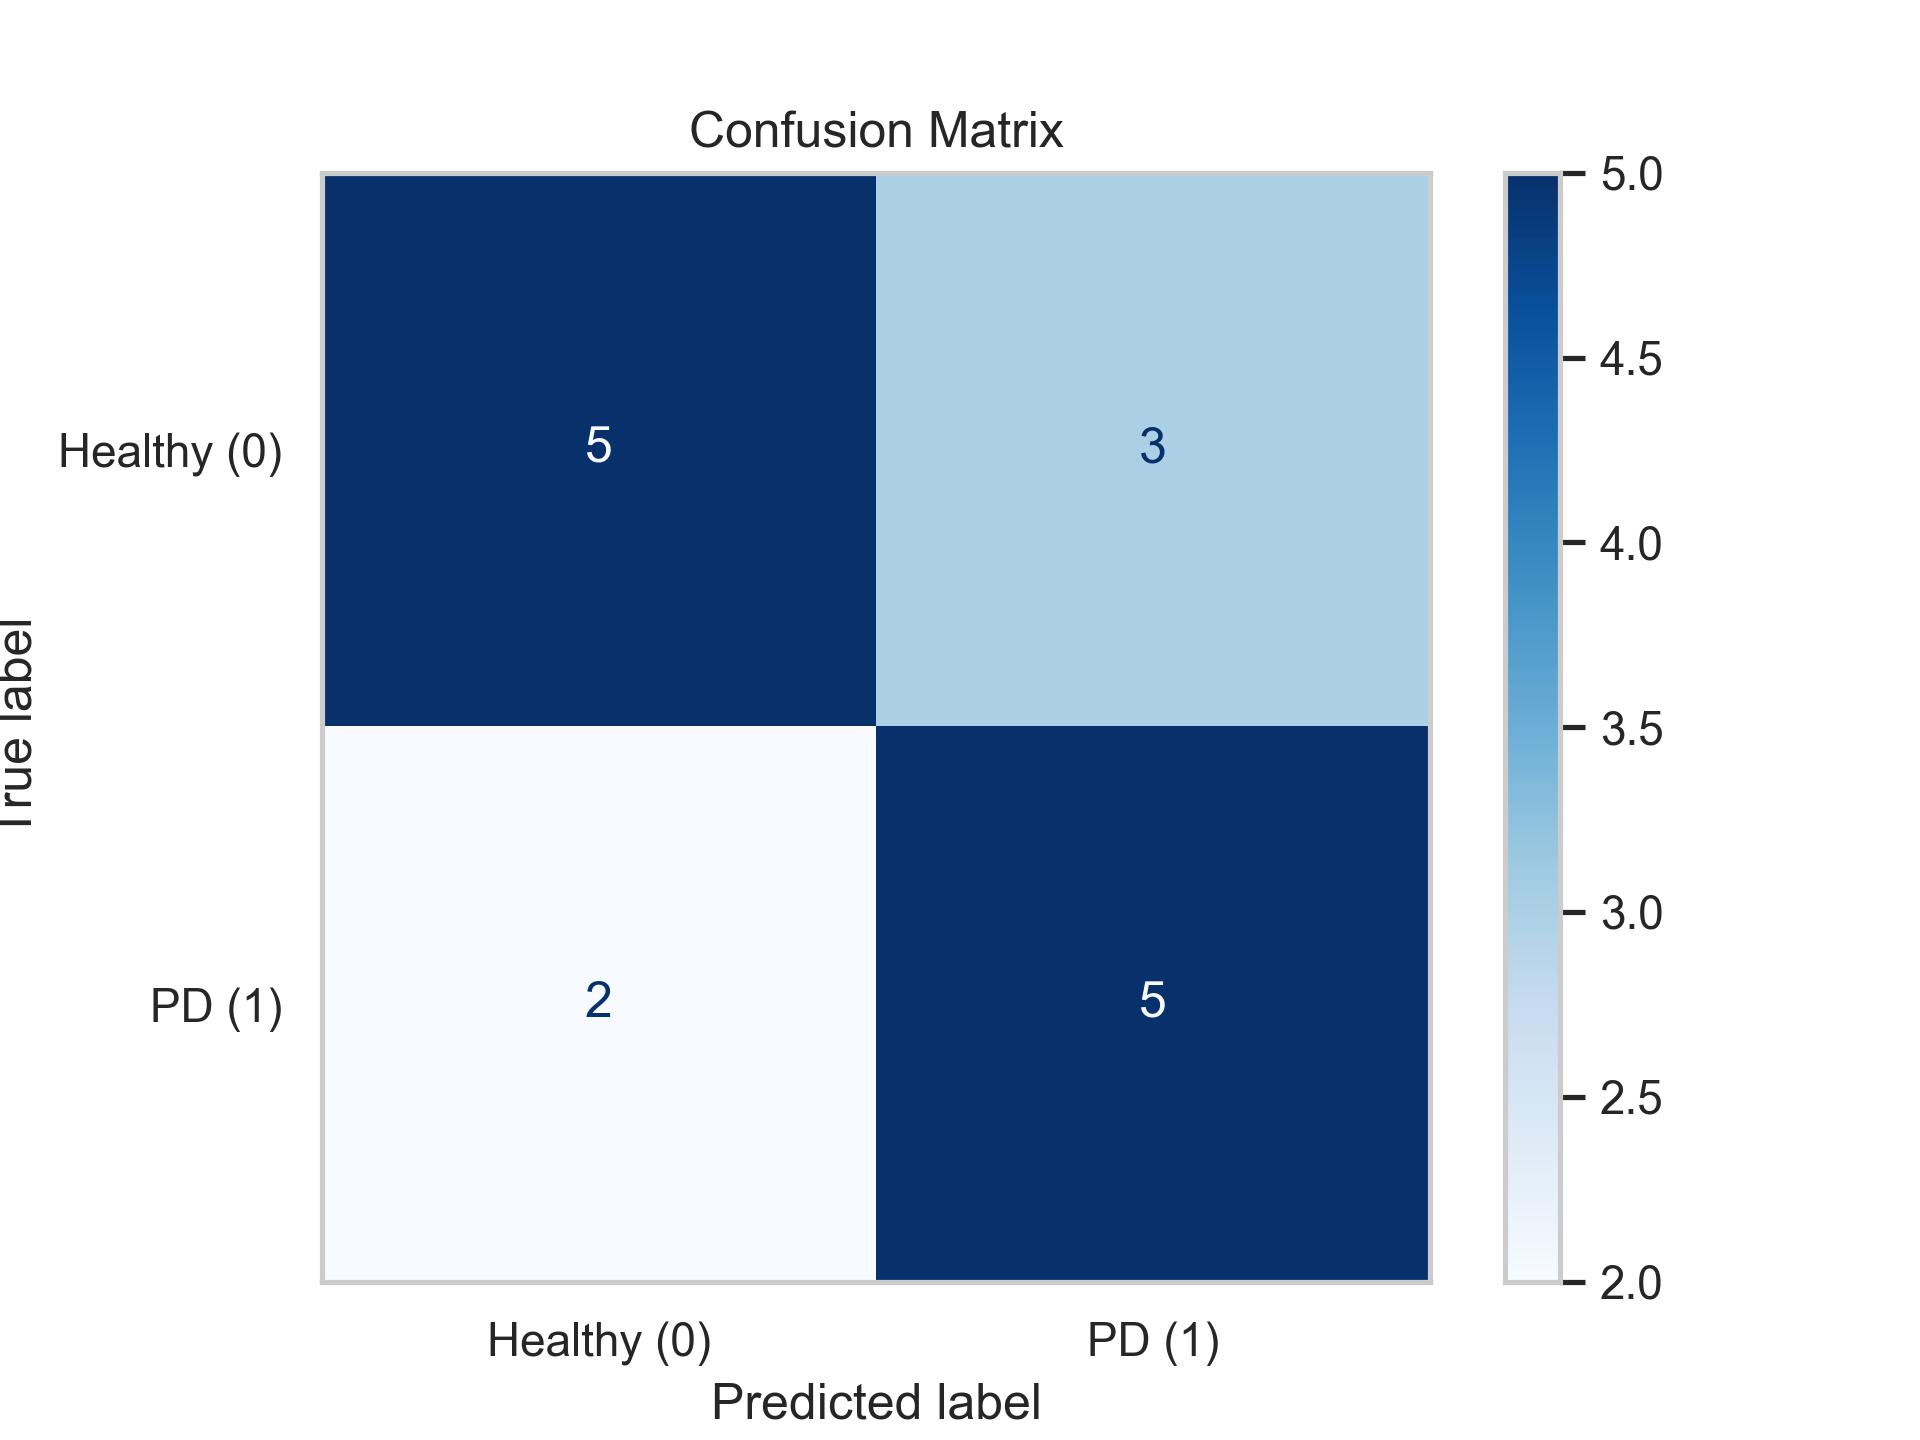
\includegraphics[width=\textwidth]{confusion_matrix.png}
        \caption{Confusion Matrix on the hold-out test set.}
        \label{fig:confusion_matrix}
    \end{minipage}\hfill
    \begin{minipage}{0.48\textwidth}
        \centering
        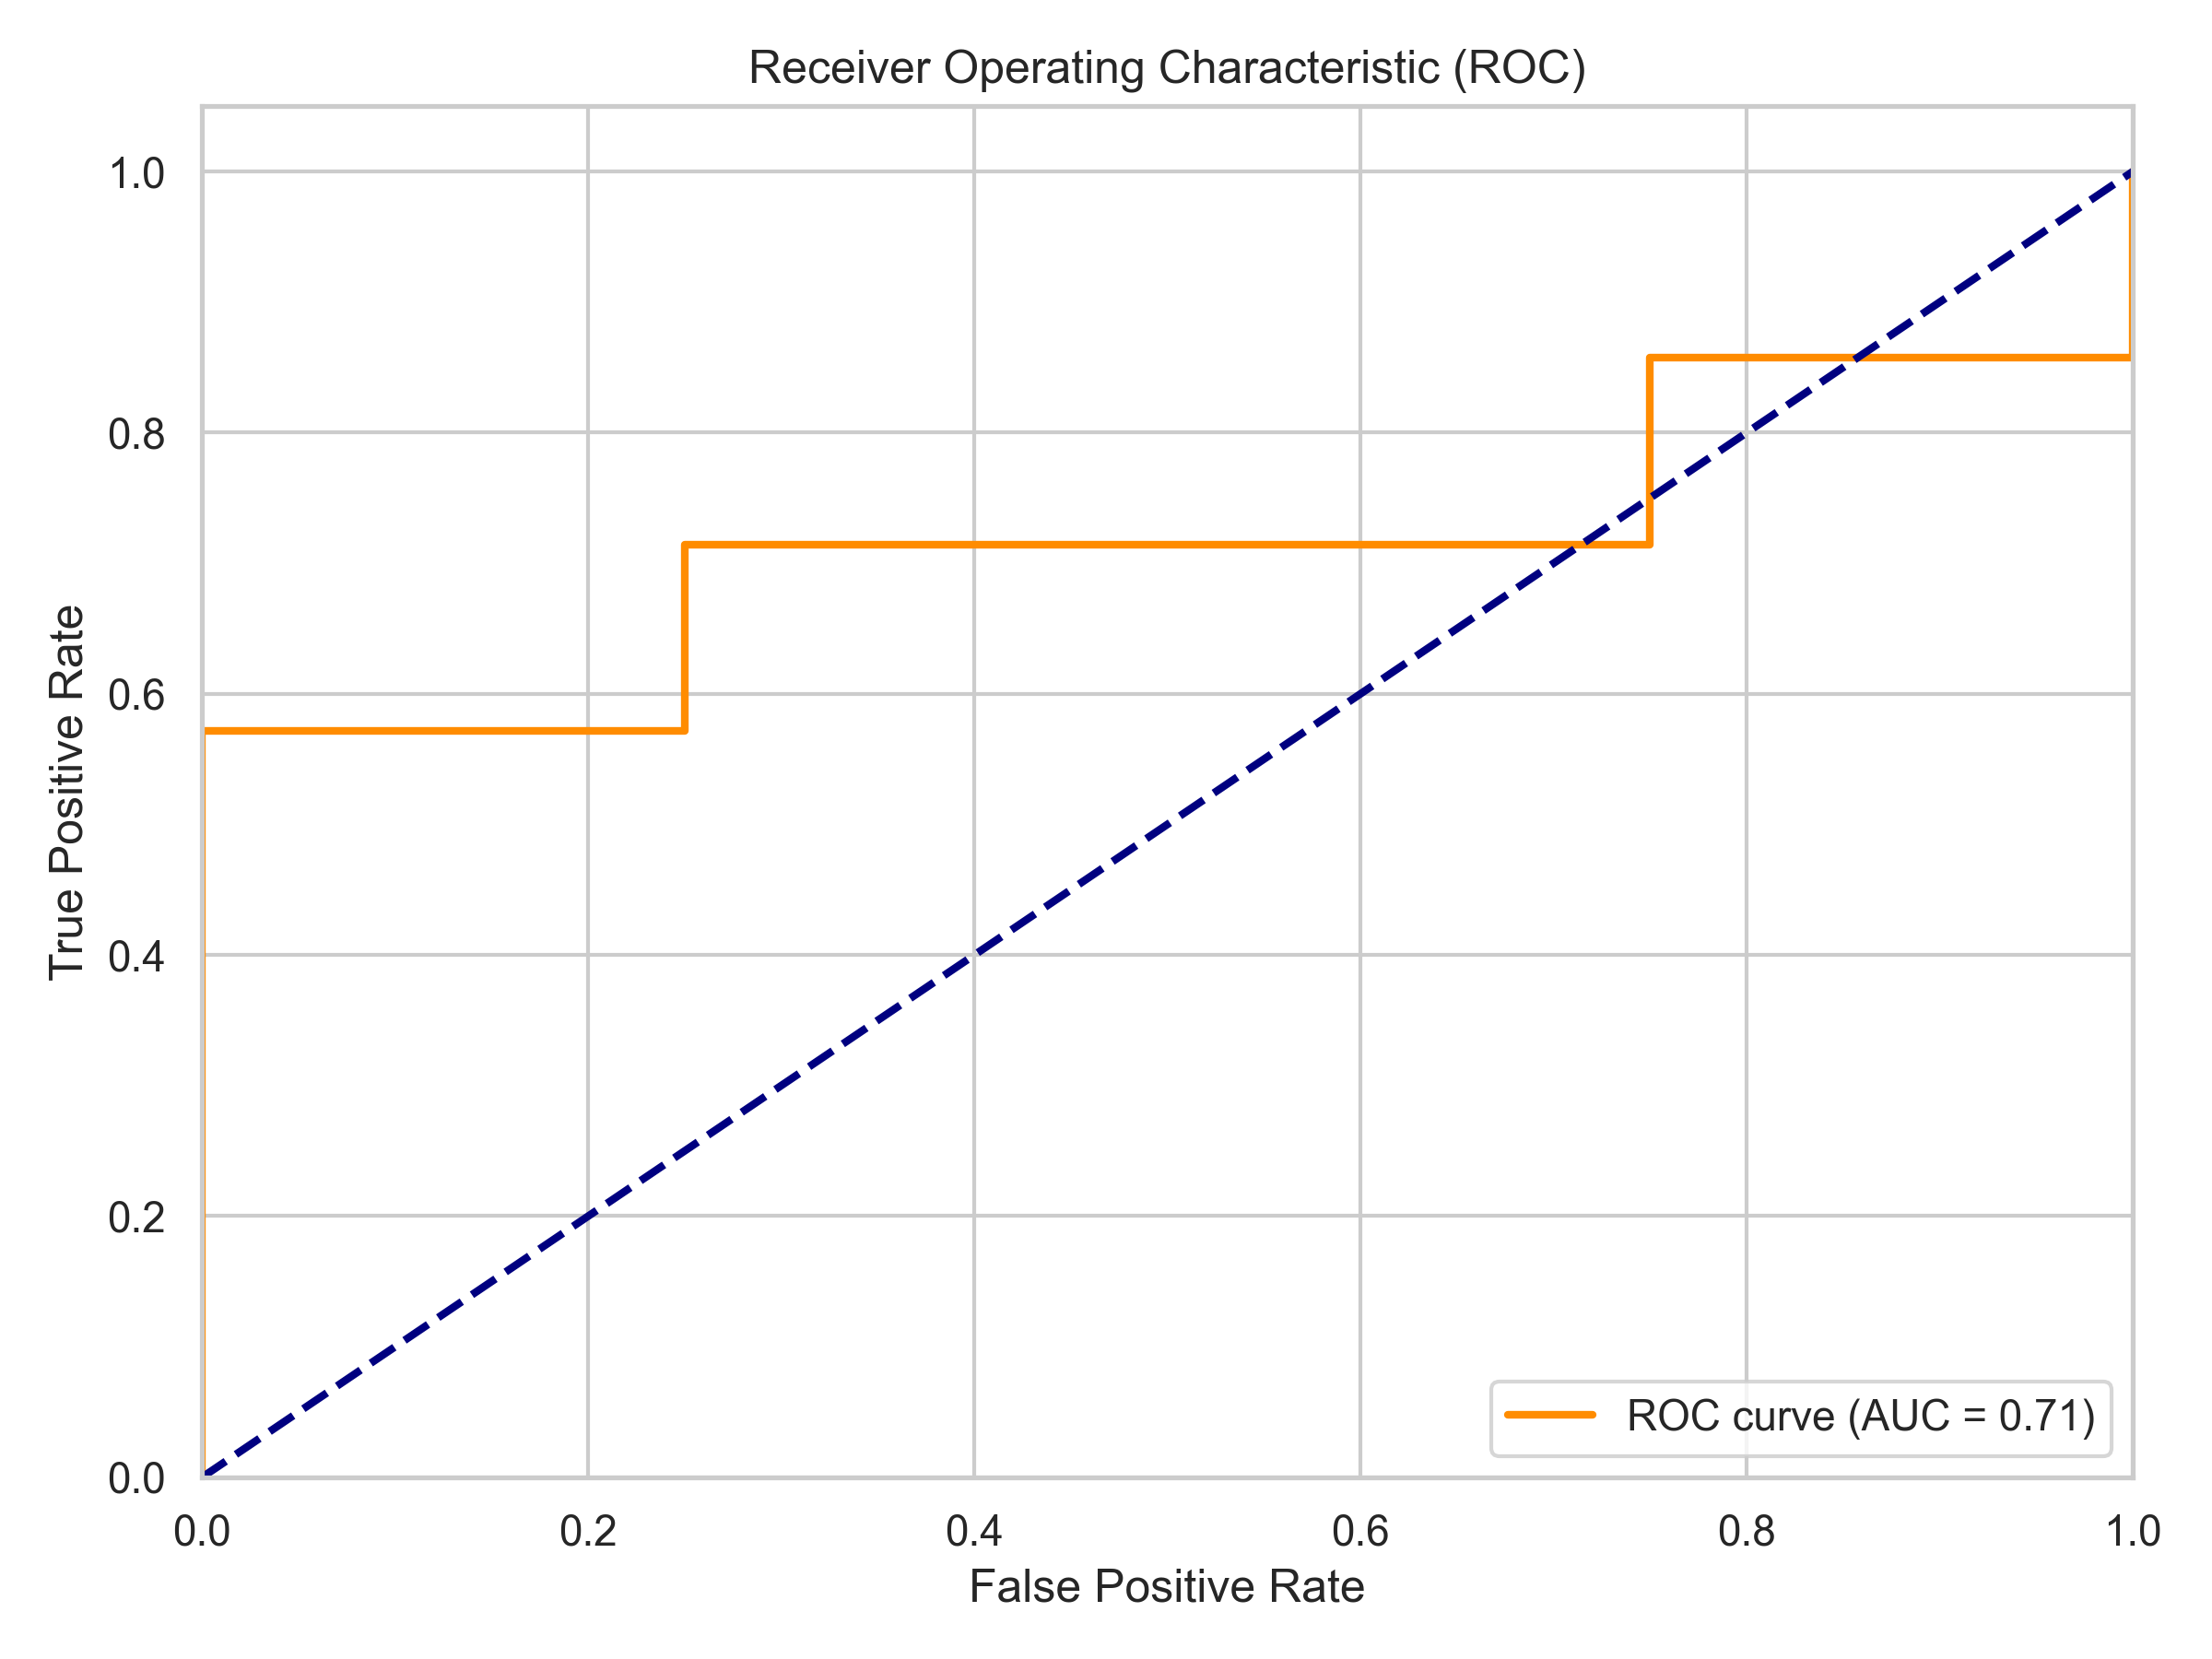
\includegraphics[width=\textwidth]{roc_curve.png}
        \caption{ROC Curve demonstrating the model's diagnostic ability.}
        \label{fig:roc_curve}
    \end{minipage}
\end{figure}
\section{Conclusion}
This project successfully establishes a solid baseline for PD classification using global statistical time-series aggregates. The Random Forest model achieved competitive performance without the need for complex deep learning architectures. Future improvements could involve employing Convolutional Neural Networks on Spectrogram representations of the time series to capture more intricate temporal dependencies and potentially improve overall F1-Score and AUC.

\end{document}